\documentclass[12pt, a4paper,oneside, openany]{book}
%fuente12pt,tamaño carta,una cara,quitar hojas en blanco,tipo libro
\usepackage[utf8]{inputenc} %fuente Unicode
%\usepackage[margin=-0cm]{geometry} %margen
\usepackage{graphicx} %uso de imagenes
\usepackage{multicol} %uso de multicolumnas
\usepackage{multirow} %multi celdas
\usepackage{lastpage} %n.total de paginas
\usepackage{colortbl} %columnas de color
\usepackage{tikz, tikz-3dplot} %figuras
\usepackage{tkz-euclide}
\usepackage{adjustbox} %manejo de margenes
\usepackage[spanish]{babel} %lenguaje español
\usepackage[document]{ragged2e} %alineacion
\usepackage[T1]{fontenc} %codificacion fuente
\usepackage{enumerate} %viñeta numeros
\usepackage{palatino} %fuente
\usepackage[colorlinks,linkcolor=myblue,citecolor=mygreen]{hyperref} %link personalizado
%-----------------------------------------------------------------
\definecolor{myblue}{HTML}{2D74B5} %color de titulos y subtitulos
%-----------------------------------------------------------------
\graphicspath{ {img/} } %localizacion de carpeta con imagenes
\renewcommand{\baselinestretch}{1.2} %espacio entre parrafos

%\AtBeginDocument{\AtBeginShipoutNext{\AtBeginShipoutDiscard}}
%elimina paginas adicionales que se agregan con el uso de hyperref
\usepackage{multirow} %multi celdas en tablas
\usepackage{longtable} %tablas multipagina
\usepackage{caption} %ajuste de tablas, figuras
\usepackage{color} %colores de texto
\usepackage{wrapfig} %rodear imagenes
\usepackage{booktabs, multirow} %bordes y rangos
\usepackage{titlesec} %titulos personalizados
\usepackage{eso-pic,picture} %imagenes con texto
\usepackage{nomencl} %simbolos de nomenclatura
\usepackage{lipsum} %crea texto default
\makenomenclature %tamaño nomenclatura
%\usepackage{showframe} %muestra el margen de las pg
%-----------------------------------------------------------------
%codigo del borde
\AddToShipoutPicture{%
\setlength\fboxsep{1pt}%
\put(24pt,24pt){\framebox(19.3066cm,28.0066cm)[lb]{}}%
}

%margenes
\usepackage{geometry}
\newgeometry{
        top=0.001in,
        bottom=3.2in,
        outer=0.55in,  %izquierda
        inner=0.55in, %derecha
        }
%-----------------------------------------------------------------
\usepackage{fancyhdr}%uso de encabezado y pie personalizado
\pagestyle{fancy}

\setlength{\headheight}{160pt}%ubicacion de caja de encabezado

\titlespacing{\chapter}{0pt}{-42pt}{0.5cm}%config capitulos, espacio de chapter
\titleformat{\chapter}[display]
{\sffamily\color{myblue}} {
    {\normalfont\color{myblue}\Large}
        \hspace{0pt}
            {\setlength\fboxsep{0pt}
                \colorbox{myblue}{
                }
            }
    }
{0 pt}
{\titlerule[0pt]\LARGE\sffamily}

%%%%%%%%%%%%%%%%%%%%%%%%%%%%%%%%%%%%%%%%%%%%%%%%%%%%%%%%%%%%%%%%%%%%%%%
\fancyhf{}%Declaración de encabezado
\pagestyle{fancy}
\fancypagestyle{plain}{}%encabezado general

\begin{document}%inicio de documento

\lhead{

\begin{minipage}{0.1\textwidth}
\scalebox{1}[1.2]{
\begin{tabular}{|m{2cm}|m{10.8cm}|m{1.0cm}|m{1.0cm}|m{1.0cm}| }

\hline

\multirow{3}{2cm}{\centering
\includegraphics[width=0.88\textwidth]{tjacdmx_logo.png}}
& \footnotesize\centering\bf\sffamily{TRIBUNAL DE JUSTICIA ADMINISTRATIVA DE TABASCO}
& \footnotesize\bf\sffamily{Día}
& \footnotesize\bf\sffamily{Mes}
&\footnotesize\bf\sffamily{Año}
\\ \cline{2-5}

& \centering\bf\footnotesize\sffamily{DIRECCIÓN GENERAL DE ADMINISTRACIÓN}
& \footnotesize\bf\sffamily{27}
& \footnotesize\bf\sffamily{02}
& \footnotesize\bf\sffamily{2023}
\\ \cline{2-5}

& \centering\bf\footnotesize\sffamily{DIRECCIÓN DE INFORMÁTICA}
& \multicolumn{3}{ |c| }{\bf\footnotesize\sffamily{Versión: 001 }}
\\ \cline{2-5}

&
\centering\bf\footnotesize\sffamily{MANUAL DE USUARIO}
& \multicolumn{3}{ |c| } {\bf\footnotesize\sffamily{Página \thepage~de\ \pageref{LastPage}}}
\\ \hline

\end{tabular}}
\end{minipage}

}
%-----------------------------------------------------------------

\centerline{
\includegraphics[width=0.8\textwidth]{tjacdmx_logo.png}}%imagen de logo en portada
%titulo de portada

\vspace{1cm}%espacio
%-----------------------------------------------------------------
\begin{flushright}%alineación a la derecha

\newcommand{\ProjectTitle}

\vspace{0cm}
%titulo en portada
{\color{myblue}{\sffamily\large\bf\sffamily
ACTUARIA V3.0 \\
CITAS SCO\\
\vspace{0.3cm}
MANUAL DE USUARIO\\
\vspace{0.2cm}
DIRECCIÓN DE INFORMÁTICA}
}

\end{flushright}
%-----------------------------------------------------------------
%pie de todas las paginas
\cfoot[]{
{\tiny
\scalebox{1}[1.2]{%tamaño de celdas
\centering\begin{tabular}{|m{4cm}|m{4.0cm}|m{4.0cm}|m{4.0cm}| }

\hline

\centering\sffamily IDENTIFICACIÓN
& \centering\sffamily ELABORÓ
&  \centering\sffamily REVISÓ
& AUTORIZÓ
\\
\hline

\centering\sffamily TJACDMX DI MANUAL USUARIO
&  \centering\sffamily Dirección de Informática
&  \centering\sffamily Dirección de Informática
&  Comité Técnico Interno de Administración de Documentos del
TJACDMX en su sesión...
\\
\hline
\end{tabular}}

}}
%-----------------------------------------------------------------


\renewcommand{\headrulewidth}{0pt}%sin linea por default
\begin{quote}%alineacion de texto

\tableofcontents

\chapter{\large{Objetivo}}\label{chap:objetivo}
Con la finalidad de ofrecer a los servidores públicos del Tribunal de Justicia Administrativa de Tabasco
una herramienta que facilite la operación de los apartados que integran el módulo
de «Actuaría v 3.0», se elaboró el presente Manual.

\chapter{\large{¿Cómo ingresar a Actuaría v3.0?}}\label{chap:ingreso}

1.Ingresaremos al Sistema con el siguiente link:

\begin{center}
\href{https://sidj.tjacdmx.gob.mx}{https://sidj.tjacdmx.gob.mx}
\end{center}

2.Nos ubicaremos en el menú y daremos clic en  {\bf{
<<Actuaria v3.0>> }}

\begin{center}
    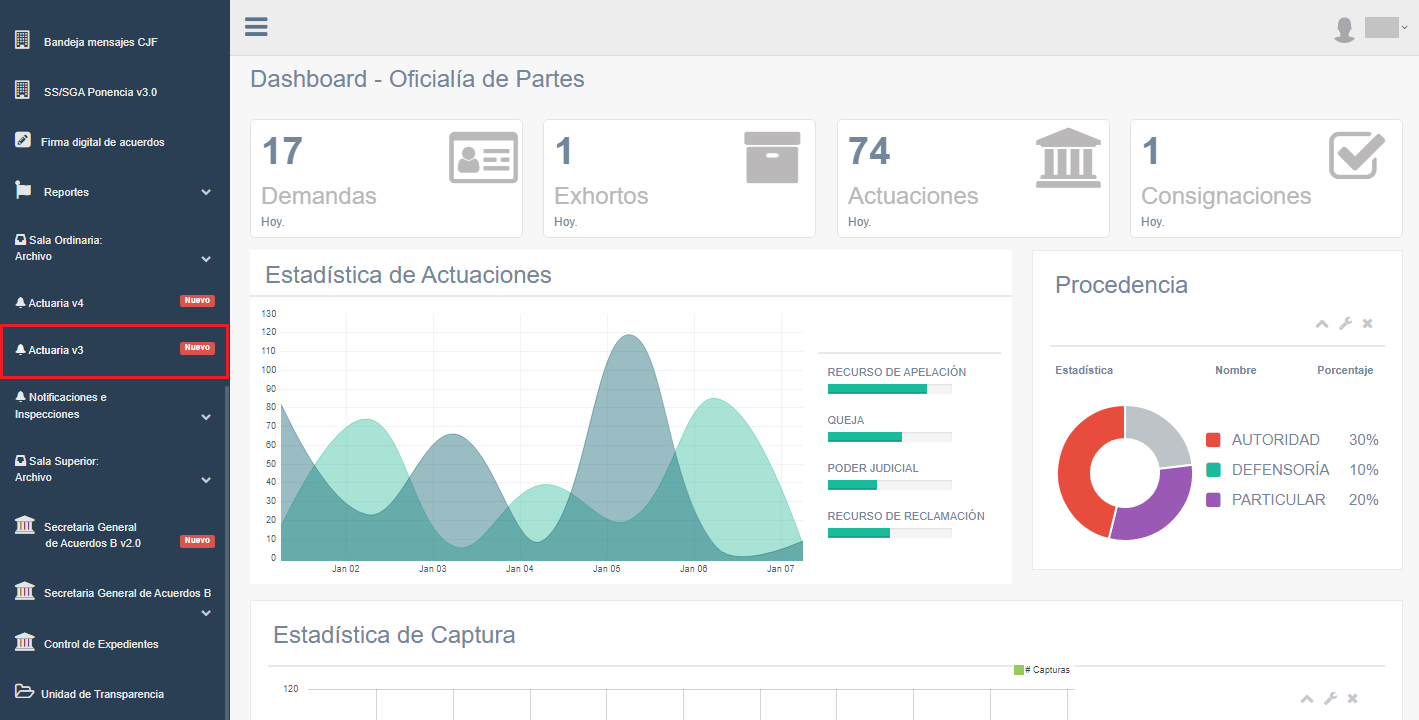
\includegraphics[width=0.88\columnwidth]{inicioAc.png}
\end{center}

\newpage
\chapter{\large{Citas SCO.}}\label{}

En el Sistema de Citas para la Oficialía, podrá realizar las siguientes actividades:

\begin{itemize}
    \item Buscar cita SCO.
    \item Información cita.
    \item Imprimir acuses.
    \item Descargar acuses.
    \item Cancelar cita.
    \item Reporte PDF.
    \item Reporte EXCEL.
\end{itemize}


{\Huge{\color{myblue} \section{¿Cómo realizar una búsqueda de citas?}\label{sec:30.1}}}

Para poder realizar la búsqueda de citas es necesario contar con al menos uno de los siguientes datos:

\begin{itemize}
    \item Número de folio de cita.
    \item Fecha de cita.
\end{itemize}

\begin{center}
    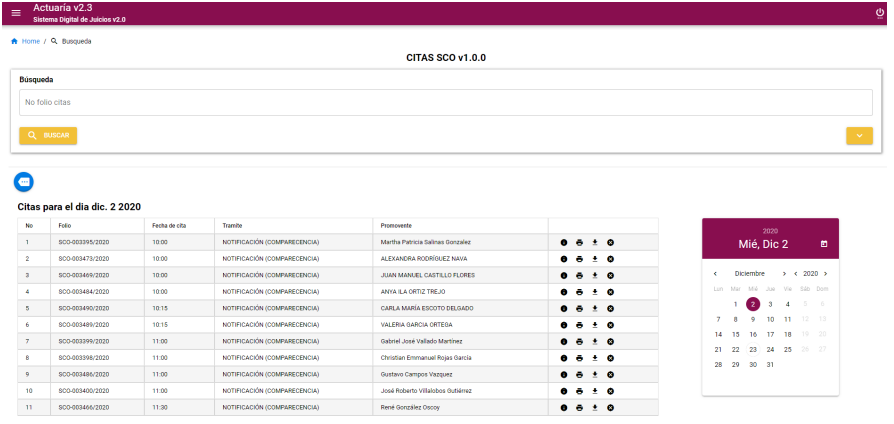
\includegraphics[width=0.88\columnwidth]{C50.png}
\end{center}

Para obtener una búsqueda más avanzada y precisa de clic en el botón identificado con el {\bf{número 1}} y se mostrará la siguiente pantalla:

\begin{center}
    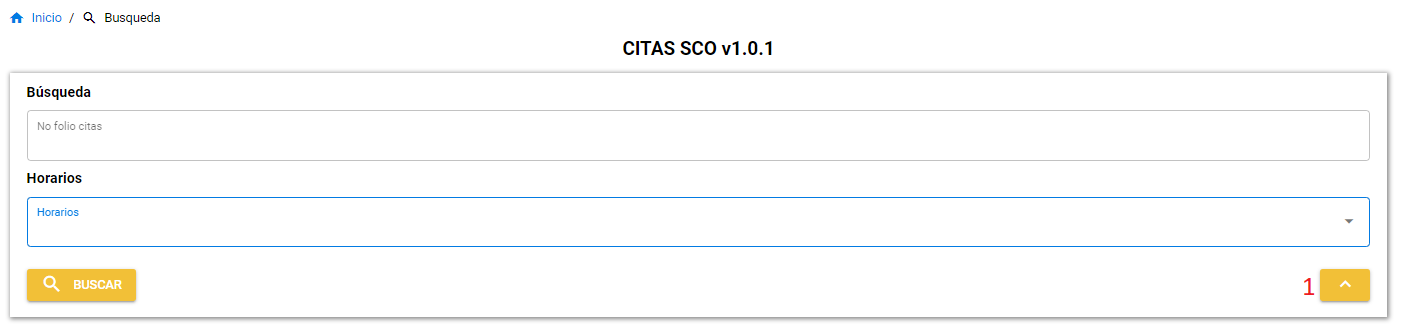
\includegraphics[width=0.88\columnwidth]{citas.png}
\end{center}

La cual contiene el campo para seleccionar los tipos de horarios

Seleccionado el tipo de horario da clic el botón de {\bf «BUSCAR»}, para que realice la búsqueda y
muestre los resultados obtenidos por el sistema.\\


{\Huge{\color{myblue} \section{Iconos}\label{sec:30.2}}}
{\bf {Descripción de las acciones de cada icono:}}

1. Información cita.

\begin{center}
    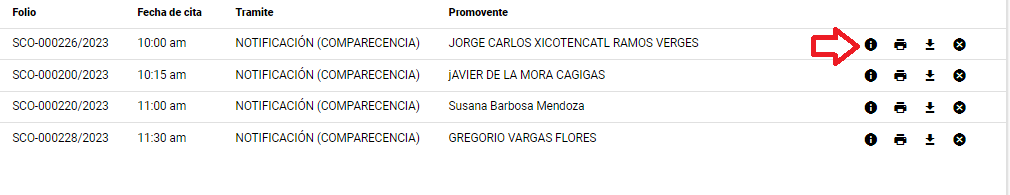
\includegraphics[width=0.88\columnwidth]{citassci.png}
\end{center}


Para visualizar la información de la cita da clic en el icono de {\bf{<<Información>>}} y se mostrara una pantalla similar.

\begin{center}
    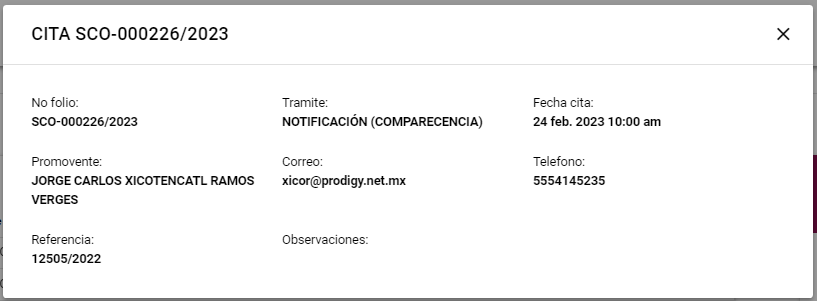
\includegraphics[width=0.75\columnwidth]{inf.png}
\end{center}

2. Imprimir acuses

Para imprimir un acuse da clic sobre el icono {\bf{<<Imprimir>>}}

\begin{center}
    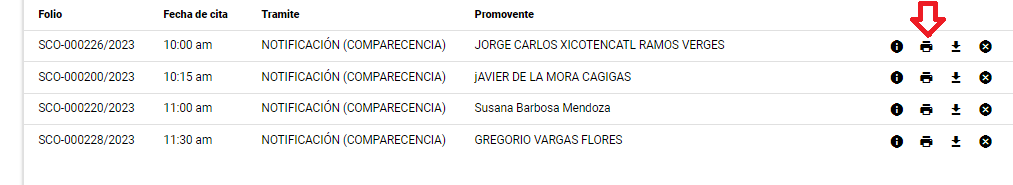
\includegraphics[width=0.75\columnwidth]{imprimiracuse.png}
\end{center}

Se mostrará la ventana de impresión, da clic en el botón {\bf «Imprimir»}.
\begin{center}
    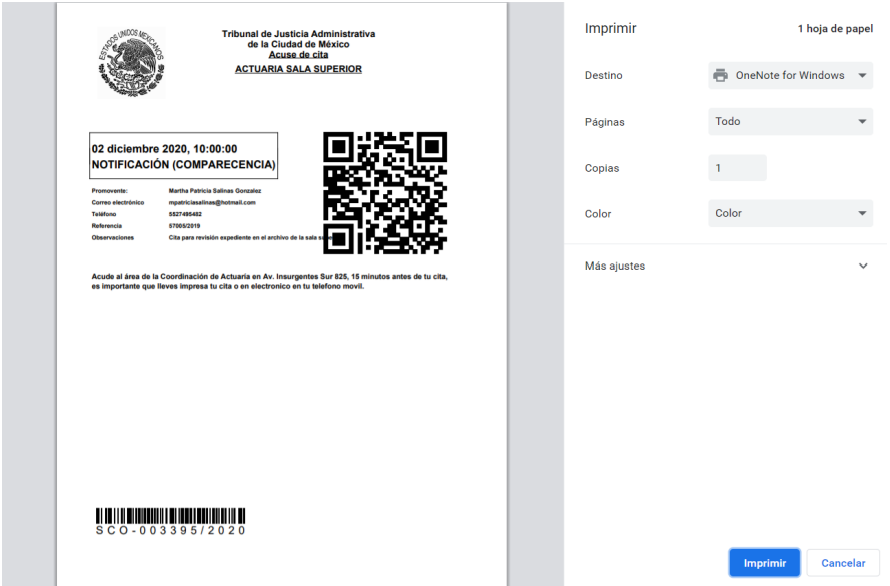
\includegraphics[width=0.8\columnwidth]{C54.png}
\end{center}

\newpage
3.Descargar acuses\\
La descarga de acuses de la cita se realiza dando clic en el icono {\bf{<<Descargar>>}} 
\begin{center}
    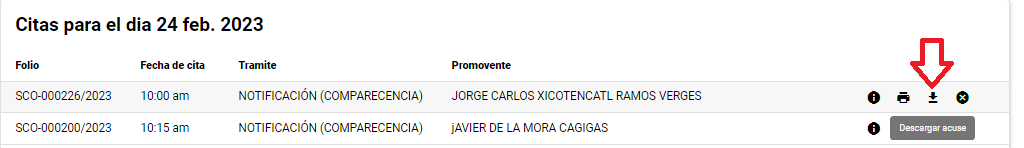
\includegraphics[width=0.88\columnwidth]{descargar_A.png}
\end{center}
El archivo se descargará en su equipo.

\vspace{1cm}

4. Reportes de citas

Para poder generar reporte de citas da clic en el icono señalado, mostrara que tipo de reporte.

\begin{itemize}
    \item Reporte PDF.
    \item Reporte EXCEL.
\end{itemize}

\begin{center}
    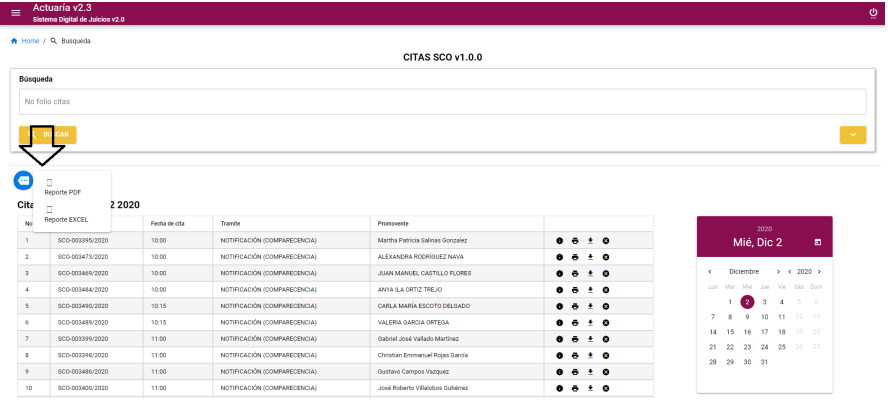
\includegraphics[width=0.88\columnwidth]{C56.png}
\end{center}

Al seleccionar el tipo de reporte, la descarga comenzara automáticamente, lo mostrara en la barra
de descargas.

\begin{center}
    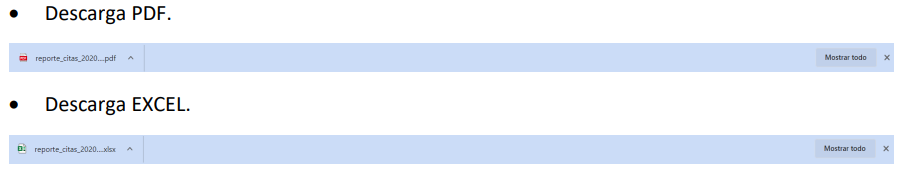
\includegraphics[width=0.88\columnwidth]{C57.png}
\end{center}

\newpage
\begin{table}[t]
\begin{center}
\begin{tabular}{| c | c | c | c | }
\hline

\multicolumn{4}{ |c| }{\cellcolor[gray]{0.9}CONTROL DE VERSIONES} \\ \hline
Versión &               Elaborado por:          & Fecha de última modificación          & Motivo \\ \hline
1.0.1   & Esthefania Vidal Solares        &      12/octubre/2022
&Creación \\ \hline
1.0.2   & Esthefania Vidal Solares        &     27/febrero/2023
&Actualización \\ \hline
\hline
\end{tabular}
\caption{Control de Versiones}
\label{tab:versiones}
\end{center}
\end{table}

\end{quote}

\end{document}